\section{Results and discussions}

\subsection{Baseline model}
The model was fitted on the reference sets and tested on the query sets for both the seen and unseen players.
Note that this model does not need any training, so we do not use the training set. The model's performance is therefore not expected to be better on the seen players when we ignore the fact there are fewer players to predict from there.
We ran the tests for four different settings of the hyperparameter $N$ (the number of moves considered). 
The results are summarized in table \ref{tab:Baseline_model}.

\begin{table}[h]
    \centering
    \caption{Baseline model results}
    \begin{tabular}{cccccccc}
        \toprule
        $n$ & \multicolumn{3}{c}{\textbf{Seen players}} & & \multicolumn{3}{c}{\textbf{Unseen players}} \\
        & Random guess & Baseline accuracy & $\frac{\text{Model}}{\text{Random}}$ & &  Random guess & Baseline accuracy & $\frac{\text{Model}}{\text{Random}}$ \\
        \midrule
        5 & 0.25\% & 3.80\% & 15.18 & & 0.0535\% & 1.54\% & 28.88\ \\
        10  & 0.25\% & 3.29\% & 13.16 & & 0.0535\% & 1.67\% & 31.2 \\
        15  & 0.25\% & 3.03\% & 12.12 & & 0.0535\%& 1.58\% & 29.48 \\
        20  & 0.25\% & 2.86\% & 11.42 & & 0.0535\% & 1.44\% & 26.94 \\
         \bottomrule
    \end{tabular}
    \label{tab:Baseline_model}
\end{table}



\subsection{Convolutional LSTM}
The model was trained for 40 epochs (100 iterations per epoch) using $n = 10$ and $n = 20$ (i.e., using the first 10 and 20 moves) and inferred on both the \emph{seen} and \emph{unseen} players. They all had $N = 40$ and $M = 20$. Additionally, the model was trained on 5 random moves from the first 20 and 10 random moves from the first 20 (for 15 and 40 epochs, respectively). One of the trained models was used using $N = 10$ and $M = 10$, meaning that in the training sampling, 10 players were sampled along with 10 games from each of the players. That model was trained for 100 epochs since it sees fewer players per batch.
\medskip\par 
Due to extreme training time and limited project time, the model training could not be fully finalized and tuned, as one epoch took 12-16 minutes. The long training times also made it neccesary to split the training up into multiple instances. Therefore, the loss plots were lost in the process. It would be possible to reconstruct them, but since there were multiple models trained, it would be a hard task. Due to limited resources, the training loss was still decreasing when the training was stopped. Table \ref{tab:conv_lstm} summarizes the results from each of the different models. We note that our best model (the one with $n = 10, N = 40, M = 20$) has 13.4\% accuracy, over 53 times better than a random guess, of predicting who is playing out of a 400-player pool of \emph{seen} players, compared to 3.8\% accuracy at best from the baseline model. The unseen player's accuracy of the LSTM model was 2.73\%, over 51 times better than a random guess, compared to 1.67\% accuracy of the best baseline model. These results show that we were able to obtain some signal from the data.

\begin{table}[ht]
    \centering
    \caption{Convolutional LSTM results}
    \begin{tabular}{cccccccccccc}
        \toprule
        $n$ & Type& $N$ & $M$ & Epochs & \multicolumn{3}{c}{\textbf{Seen players}} & & \multicolumn{3}{c}{\textbf{Unseen players}} \\
        & & & & & Random & Accuracy & $\frac{\text{Model}}{\text{Random}}$ & &  Random & Accuracy & $\frac{\text{Model}}{\text{Random}}$ \\
        \midrule
        5 & random & 40 & 20 & 15 & 0.25\% & 2.1\% & 8.4 & & 0.0535\% & 1.54\% & 8.92\ \\
        10 & first & 40 & 20 & 40 & 0.25\% & 13.4\% & 53.40 & & 0.0535\% & 2.73\% & 51.14 \\
        10 & first & 10 & 10 & 100 & 0.25\% & 8.82\% & 35.28 & & 0.0535\% & 1.89\% & 35.46 \\
        10 & random & 40 & 20 & 40 & 0.25\% & 8.58\% & 34.34 & & 0.0535\% & 1.93\% & 36.12 \\
        20 & first & 40 & 20 & 40 & 0.25\% & 12.9\% & 50.83 & & 0.0535\% & 2.24\% & 42.06 \\
         \bottomrule
    \end{tabular}
    \label{tab:conv_lstm}
\end{table} 

\newpage
\subsubsection{Comparison to Previous Work}
In their work, \cite{main_article} used similar hyperparameters to those that were used in this project, i.e. $N = 40$ and $M = 20$ for the training sampling. They used architecture similar to the one used in this project as well. However, their model was transformer-based. Their main model was trained on Lichess data from players between 1000-2000 Lichess points, each having played over 10000 games, while in this project, only elite players were used (players with 2400 points or more). They however also trained a model on elite players, which can be found in the appendix of their article. It is quite hard to read what their results were from their experiments with a model for the high ranked players. From what can be seen in the appendix, they seem to have obtained a baseline accuracy of over 60\% in a pool of around 1600 players, while their high ranking player model obtained accuracy of only 29.8\% for \emph{seen} players (1600 player pool) and 29.5\% for their \emph{unseen} players (408 player pool). These results are quite different to ours, our baseline model, which was constructed similarily to their baseline, was performing much worse than our LSTM model, while it is the other way around in their article. This might point to some discrepancy in their studies or the result of different data being used. This difference is, however, quite large.
\medskip\par 
Judging from these results, it seems that elite players are likely to be playing in a similar manner since they most likely use computers when they are training, especially for the early moves. This classification task may therefore be harder than classifying games from worse players. \cite{main_article} also seem to have had access to considerable computing power, since our model had quite extreme running times and we were not able to train for as long nor with as much data as they did.

\subsection{Examples of Embeddings}
To visualize the inference of the model, the reference set for 8 players was passed through the trained model for $n = 10, N = 40, M = 20$, and the centroids calculated. Then, the query set for these same 8 players was passed through the model and the embeddings calculated. Finally, $t$-SNE projections were visualized as figure \ref{fig:tsne} shows. We see that the \emph{seen} player centroids are spaced apart and the embeddings of a player's game are quite close to the corresponding centroid. For the \emph{unseen} players, the clusters seem to follow this trend as well.

\begin{figure}[ht!]
    \centering
    \begin{subfigure}[t]{0.49\textwidth}
        \centering
        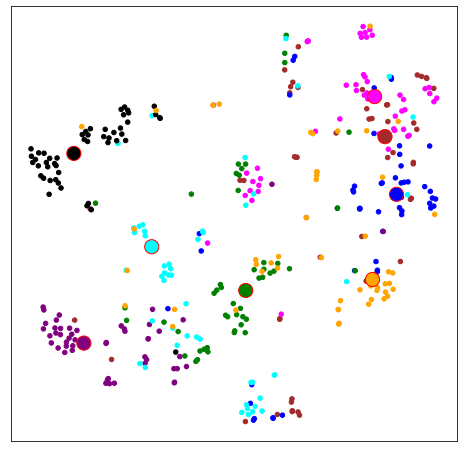
\includegraphics[width=2.5in]{figures/tsne-seen.png}
        \caption{$t$-SNE representation of games from \emph{seen} players.}
    \end{subfigure}%
    ~ 
    \begin{subfigure}[t]{0.49\textwidth}
        \centering
        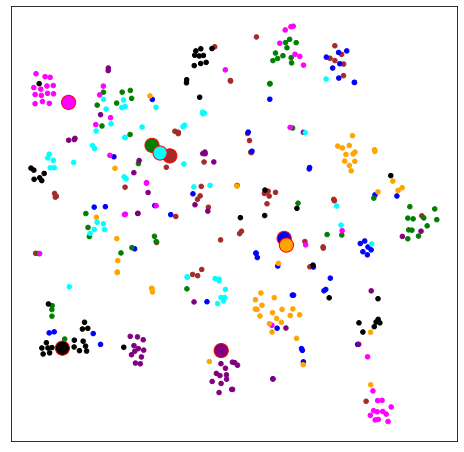
\includegraphics[width=2.5in]{figures/tsne-unseen.png}
        \caption{$t$-SNE representation of games from \emph{unseen} players.}
    \end{subfigure}
    \caption{$t$-SNE representation of chess games. The larger points with the red border represent the centroids for the reference set and the smaller points represent the embeddings of the games in the query set.}
    \label{fig:tsne}
\end{figure}
